\subsection{  Design Approach (Function oriented or Object oriented)}
A software design document (SDD) is a written description of a software product, that
a software designer writes in order to give a software development team overall guidance
to the architecture of the software project. An SDD usually accompanies an architecture
diagram with pointers to detailed feature specifications of smaller pieces of the design.
Practically, a design document is required to coordinate a large team under a single vision.
A design document needs to be a stable reference, outlining all parts of the software and
how they will work. The document is commanded to give a fairly complete description,
while maintaining a high-level view of the software.\\\\
There are two kinds of design documents called HLDD (high-level design document)
and LLDD (low-level design document). The SDD contains the following documents:\\
\begin{itemize}
\item The data design describes structures that reside within the software. Attributes and
relationships between data objects dictate the choice of data structures.
\item The architecture design uses information flowing characteristics, and maps them into
the program structure. The transformation mapping method is applied to exhibit
distinct boundaries between incoming and outgoing data. The data flow diagrams
allocate control input, processing and output along three separate modules.
\item The interface design describes internal and external program interfaces, as well as
the design of human interface. Internal and external interface designs are based on
the information obtained from the analysis model.
\item The procedural design describes structured programming concepts using graphi-
cal, tabular and textual notations. These design mediums enable the designer to
represent procedural detail, that facilitates translation to code. This blueprint for
implementation forms the basis for all subsequent software engineering worked.
\end{itemize}
\textbf{System Design} : Systems design is the process or art of defining the architecture,
components, modules, interfaces, and data for a system to satisfy specified requirements.
One could see it as the application of systems theory to product development. There is
some overlap with the disciplines of systems analysis, systems architecture and systems
engineering.\\\\
\begin{enumerate}
\item {\textbf{External design}} -External design consists of conceiving, planning out and specifying the externally
observable characteristics of the software product. These characteristics include
user displays or user interface forms and the report formats, external data sources
and the functional characteristics, performance requirements etc. External design
begins during the analysis phase and continues into the design phase.
\item {\textbf{Logical design}} - The logical design of a system pertains to an abstract representation of the data
flows, inputs and outputs of the system. This is often conducted via modeling,
which involves a simplistic (and sometimes graphical) representation of an actual
system. In the context of systems design, modeling can undertake the following
forms, including:
\begin{itemize}
Data flow diagrams
Entity Relationship Diagrams
\end{itemize}
\item {\textbf{Physical design}} - The physical design relates to the actual input and output processes of the sys-
tem. This is laid down in terms of how data is input into a system, how it is
verified/authenticated, how it is processed, and how it is displayed as output.
\end{enumerate}
It follows a object oriented design approach. object-oriented design techniques are
very popular, currently in use in many software development organizations.\\\\
Object-oriented analysis and design is a popular technical approach to analyzing, designing an application, system, or business by applying the object-oriented paradigm and visual modeling throughout the development life cycles to foster better stakeholder communication and product quality.\\\\
\subsection{SA/SD methodology}
It has essential features of several important function-oriented design methodologies. If
you need to use any specific design methodology later on, you can do so easily with small
additional effort.\\\\
Structured Analysis and Design Technique (SADT) is a diagrammatic notation designed
specifically to help people describe and understand systems.It offers building blocks to
represent entities and activities, and a variety of arrows to relate boxes. These boxes and
arrows have an associated informal semantics. SADT can be used as a functional analysis
tool of a given process, using successive levels of details. The SADT method not only
allows one to define user needs for IT developments, which is often used in the industrial
Information Systems, but also to explain and present an activitys manufacturing processes
and procedures.\\\\
Object-oriented design is the process of planning a system of interacting objects for the purpose of solving a software problem. It is one approach to software design.An object contains encapsulated data and procedures grouped together to represent an entity. The 'object interface', how the object can be interacted with, is also defined. An object-oriented program is described by the interaction of these objects. Object-oriented design is the discipline of defining the objects and their interactions to solve a problem that was identified and documented during object-oriented analysis.What follows is a description of the class-based subset of object-oriented design, which does not include object prototype-based approaches where objects are not typically obtained by instancing classes but by cloning other (prototype) objects. Object-oriented design is a method of design encompassing the process of object-oriented decomposition and a notation for depicting both logical and physical as well as state and dynamic models of the system under design.\\\\
\subsection{Detail Design}
We basically describe the functionality of the system internally. The internal design de-
scribes how data is flowing from database to the user and how they both are internally
connected. For this reason we can show the design of the system in detailed manner by
many ways:\\\\
\textbf{Flowchart:} A flowchart is a type of diagram that represents an algorithm or process,
showing the steps as boxes of various kinds, and their order by connecting them with
arrows. This diagrammatic representation can give a step-by-step solution to a given
problem. Process operations are represented in these boxes, and arrows connecting them
represent flow of control. Data flows are not typically represented in a flowchart, in con-
trast with data flow diagrams; rather, they are implied by the sequencing of operations.
Flowcharts are used in analyzing, designing, documenting or managing a process or pro-
gram in various fields.\\\\
Design standards must be set at the start of the DD phase by project management to co-
ordinate the collective efforts of the team. This is especially necessary when development
team members are working in parallel. The developers must first complete the top-down
decomposition of the software started in the AD phase (DD02) and then outline the pro-
cessing to be carried out by each component. Developers must continue the structured
approach and not introduce unnecessary complexity. They must build defences against
likely problems.\\\\
Developers should verify detailed designs in design reviews, level by level. Review of
the design by walkthrough or inspection before coding is a more efficient way of elimi-
nating design errors than testing. The developer should start the production of the user
documentation early in the DD phase. This is especially important when the HCI com-
ponent is significantly large writing the SUM forces the developer to keep the user’s view
continuously in mind.\\\\
Reuse of the software: Software reuse questions can arise at all stages of design.
In the DD phase decisions may have been taken to reuse software for all or some major
components, such as:\\\\
\begin{itemize}
\item Application generators;
\item Database management systems;
\item Human-computer interaction utilities;
\item Mathematical utilities;
\item Graphical utilities
\end{itemize}
The high-level design will normally have been identified during the AD phase. De-
tailed designs may have to be prototyped in the DD phase to find out which designs
best meet the requirements.\\\\
The feasibility of a novel design idea should be checked by prototyping. This en-
sures that an idea not only works, but also that it works well enough to meet
non-functional requirements for quality and performance.\\\\
\subsection{System Design using design tools}
A Data Flow Diagram (DFD) is a geo graphical representation of the flow of data through
an information system, modeling its process aspects. A DFD is often used as a prelimi-
nary step to create an overview of the system, which can later be elaborated. DFDs can
also be used for the visualization of data processing (structured design).\\\\
A DFD shows what kind of information will be input to and output from the system,
where the data will come from and go to, and where the data will be stored. It does not
show information about the timing of process or information about whether processes will
operate in sequence or in parallel (which is shown on a flowchart).\\\\
\begin{figure} [h]
\centering
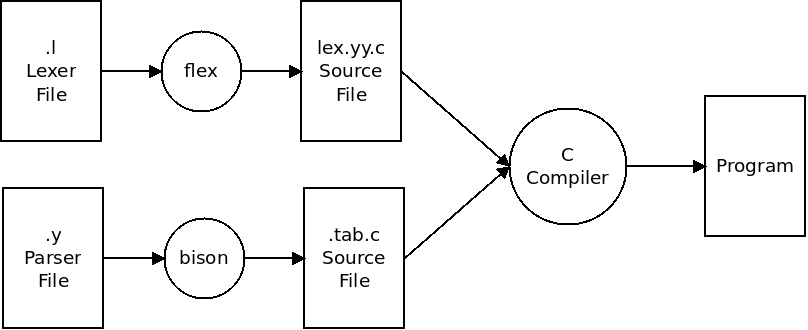
\includegraphics[scale=0.5]{images/bison.png}
\caption{Data Flow Diagram}
\end{figure}
\subsection{User Interface Design}
This project is based on Command-Line based. In this apporach not User Interface Design needs. Console Mode or command-Line based design is Text mode programs are program which output is only made out of text. In Windows terminology, they are called CUI (Console User Interface) executables, by opposition to GUI (Graphical User Interface) executables. Win32 API provide a complete set of APIs to handle this situation, which goes from basic features like text printing, up to high level functionalities (like full screen editing, color support, cursor motion, mouse support), going through features like line editing or raw/cooked input stream support.\\
Command-line interfaces to computer operating systems are less widely used by casual computer users, who favor graphical user interfaces. Command-line interfaces are often preferred by more advanced computer users, as they often provide a more concise and powerful means to control a program or operating system.\\\\
\begin{figure} [h]
\centering
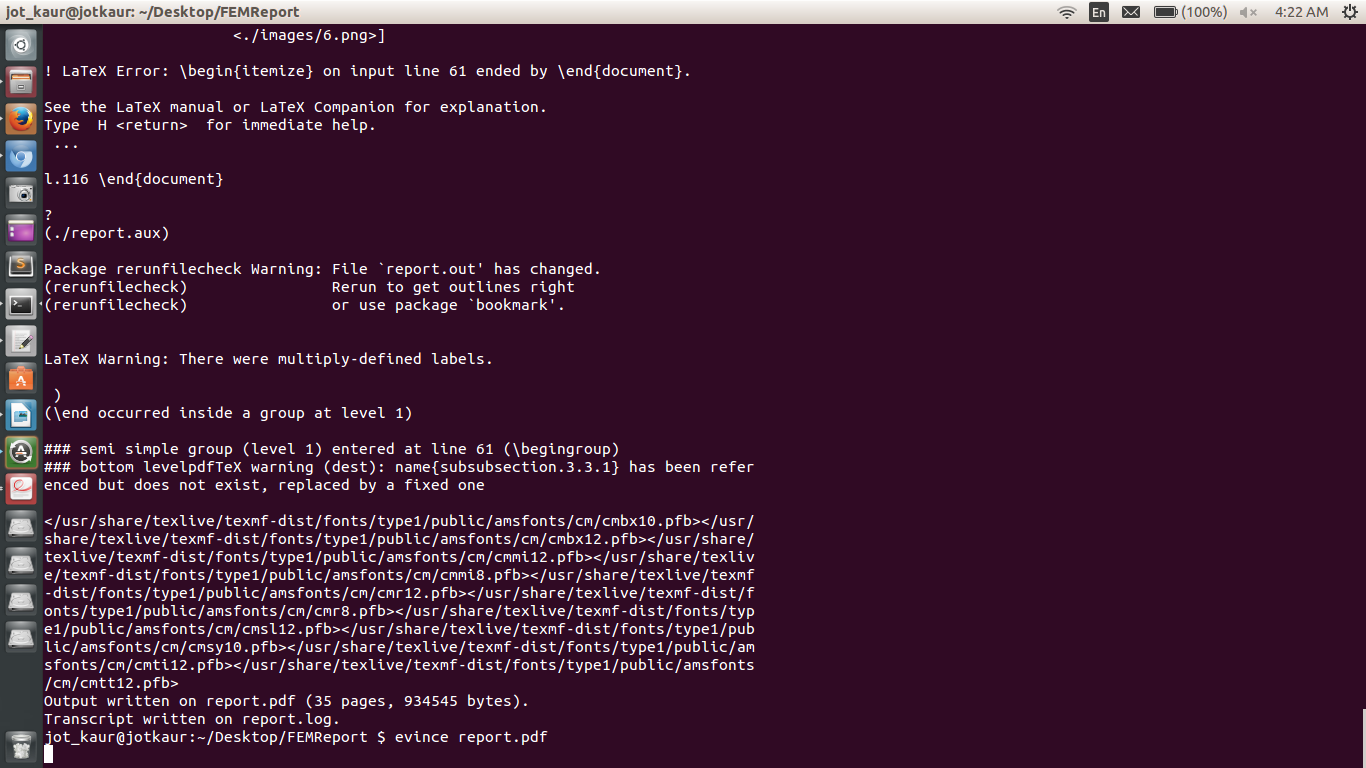
\includegraphics[scale=0.5]{images/command.png}
\caption{Console User Interface}
\end{figure}
\subsection{Methodology}
\textbf{Step 1:} Researching the needs of the students and administration and finding
out the facilities required to develop project.\\
\textbf{Step 2:} Documenting the needs and then preparing the layout for the project,
and deciding the various modules to be included in the software.\\
\textbf{Step 3:} DFDs will be prepared showing various interactions between users
and the system.\\
\textbf{Step 4:} Selecting the technology for developing the project and installing the
required tools for developing the project. We will install Net beans-IDE and
My SQL Server.\\
\textbf{Step 5:} Developing the front end- All the forms required to get users infor-
mation, informative forms etc. will be developed in html.\\
\textbf{Step 6:} Developing the back end- the tables necessary to store the data relating to customers and tables containing the data of the organization will be developed in My SQL. Tables can be updated from time to time. Efforts will be made to ensure no redundancy.\\
\textbf{Step 7:} Connectivity between front end and back end- will be used to connect
front end and back end, this will result in complete running project where user
can interact with system and can enter details which will saved at back end.
The details already entered can be updated.\\
\textbf{Step 8:} Testing the system by running it and by entering data and retrieving
it.\\






